\addcontentsline{toc}{section}{\bfseries Mở đầu}
\section*{Mở đầu}
Trong bài báo cáo này, em sẽ trình bày về mô hình nhận diện và phân loại các sản phẩm về thời trang với các bước thực hiện cụ thể là đầu tiên sẽ giới thiệu về bộ dữ liệu sử dụng cho mô hình, tiếp đến là tiền xử lý dữ liệu, xây dựng mô hình và cuối cùng là đưa ra đánh giá cho mô hình. Em rất mong nhận được góp ý của thầy để bài cáo được hoàn thiện hơn.

\indent Em xin chân thành cảm ơn thầy Trần Ngọc Thăng đã luôn nhiệt tình giảng dạy, truyền đạt những kiến thức về môn Khai phá dữ liệu để giúp em có thể hoàn thiện bài báo cáo này.

\indent Chúng em xin chân thành cảm ơn!

\begin{minipage}{0.5\textwidth}
\end{minipage}
\hspace{0.5\textwidth}
\begin{minipage}{0.5\textwidth}
	\noindent\begin{center}
		\vspace{0.5cm}
		\textit{Hà Nội, tháng 2 năm 2023}
		\textbf{}
	\end{center}	
\end{minipage}

\newpage
\renewcommand{\arraystretch}{2}

\addcontentsline{toc}{section}{\bfseries Yêu cầu bài tập cuối kỳ}
\section*{Yêu cầu bài tập cuối kỳ}
\begin{center}
    \begin{figure}[!h]
        \centering
        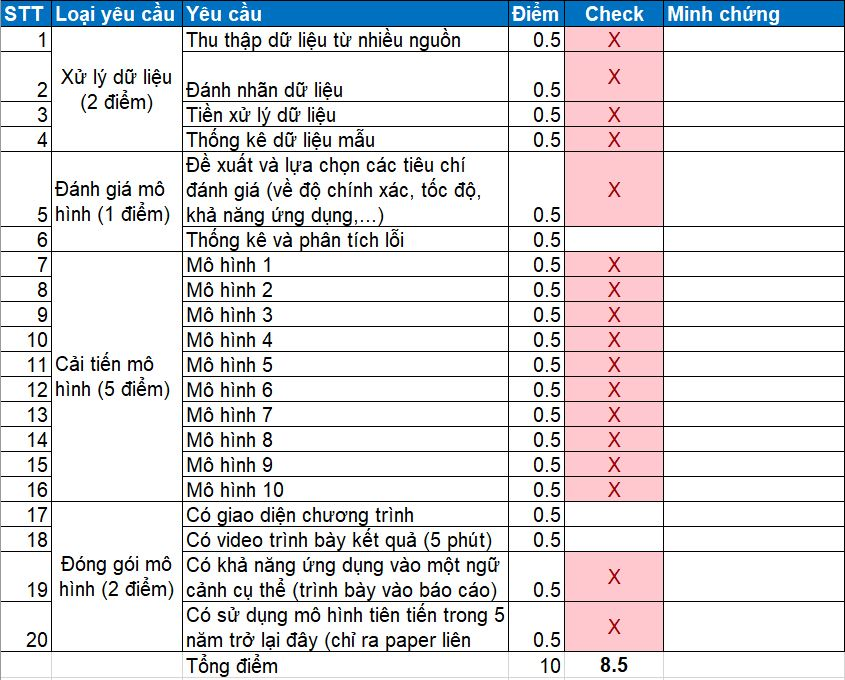
\includegraphics[scale = 1]{fileanh/yeucau.jpg}
        \caption{Checklist}
    \end{figure}
\end{center}
